%%%%%%%%%%%%%%%%%%%%%% BFS and DFS %%%%%%%%%%%%%%%%%%%%%%%%%%%%%%%%%%%%
\section{BFS and DFS}

\begin{frame}
  \frametitle{BFS and DFS}

  \begin{quote}
    \textcolor{blue}{``For fundamental achievements in the design and analysis of algorithms and data structures.''}

    \hfill {--- Turing Award 1986}
  \end{quote}

  \begin{columns}
    \begin{column}{0.50\textwidth}
      \begin{figure}
        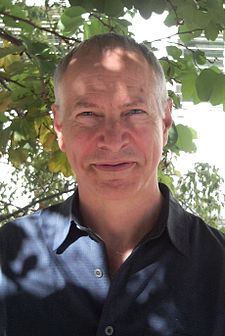
\includegraphics[scale=0.30]{figure/bfs_dfs/Tarjan}
        \caption{{\scriptsize Robert Endre Tarjan (April 30, 1948).}}
        \label{fig:Tarjan}
      \end{figure}
    \end{column}

    \begin{column}{0.50\textwidth}
      \begin{figure}
        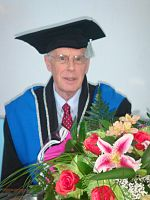
\includegraphics[scale=0.50]{figure/bfs_dfs/hopcroft}
        \caption{{\scriptsize John Edward Hopcroft (October 7, 1939)}.}
        \label{fig:hopcroft}
      \end{figure}
    \end{column}
  \end{columns}

\end{frame}


     %%%%%%%% Exploring types of edges on both BFS and DFS %%%%%%%
\subsection{Exploring Types of Edges on Both BFS and DFS}

\begin{frame}
  \frametitle{Types of edges on DFS}

  \begin{columns}
    \begin{column}{0.50\textwidth}
      \textcolor{purple}{DFS on digraph:}
      \begin{figure}
        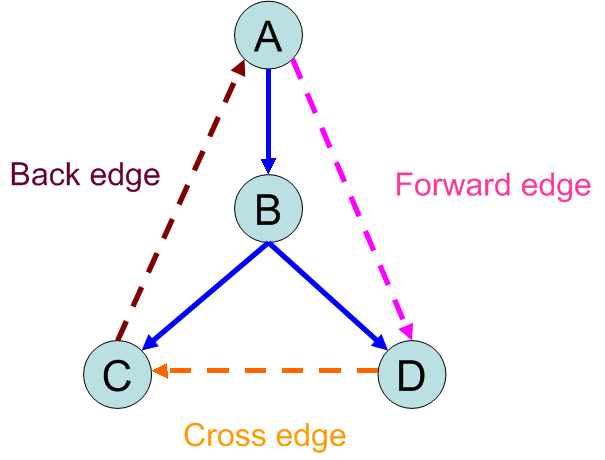
\includegraphics[scale=0.30]{figure/bfs_dfs/dfsdi}
        \caption{{\scriptsize DFS on digraph.}}
        \label{fig:dfsdi}
      \end{figure}
    \end{column}

    \begin{column}{0.50\textwidth}
      \textcolor{purple}{DFS on undirected graph  \\ ([\textcolor{blue}{$P_{380}$ 7.28}]):}
      \begin{figure}
        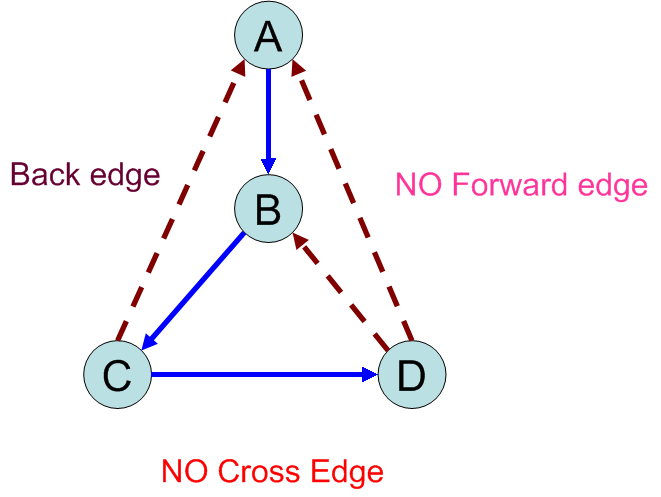
\includegraphics[scale=0.30]{figure/bfs_dfs/dfsundirected}
        \caption{{\scriptsize DFS on undirected graph.}}
        \label{fig:dfsundirected}
      \end{figure}
    \end{column}
  \end{columns}
      
\end{frame}


\begin{frame}
  \frametitle{Types of edges on BFS}

  \begin{columns}
    \begin{column}{0.50\textwidth}
      \textcolor{purple}{BFS on digraph:}
      \begin{figure}
        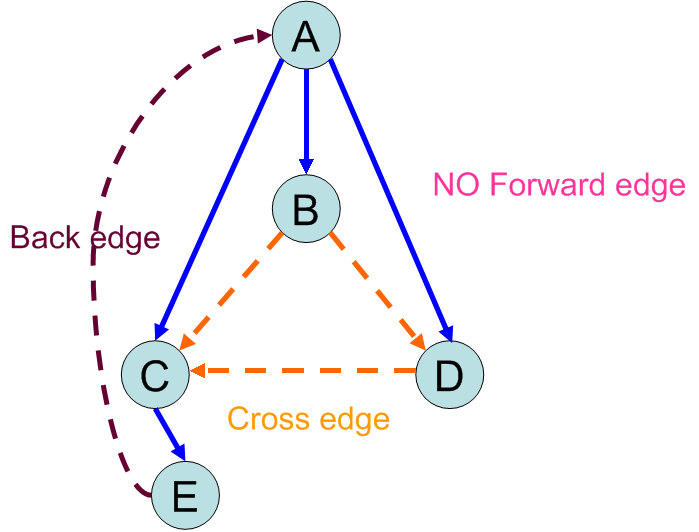
\includegraphics[scale=0.30]{figure/bfs_dfs/bfsdi}
        \caption{{\scriptsize BFS on digraph.}}
        \label{fig:bfsdi}
      \end{figure}
    \end{column}
  
    \begin{column}{0.50\textwidth}
      \textcolor{purple}{BFS on undirected graph:}
      \begin{figure}
        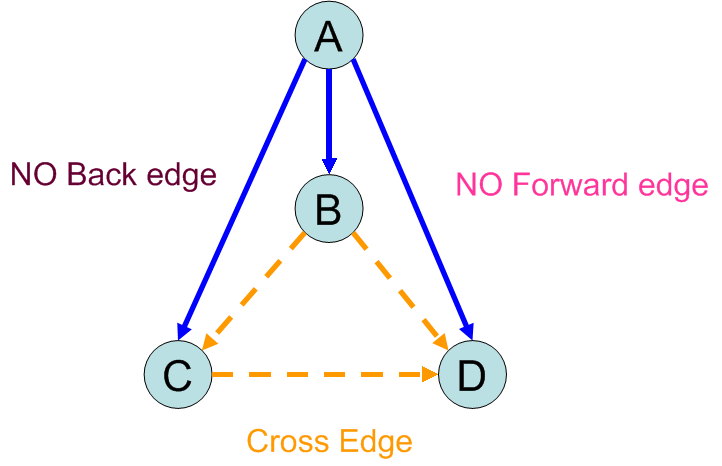
\includegraphics[scale=0.30]{figure/bfs_dfs/bfsundirected}
        \caption{{\scriptsize BFS on undirected graph.}}
        \label{fig:bfsundirected}
      \end{figure}
    \end{column}
  \end{columns}
  
\end{frame}



\begin{frame}
  \frametitle{Cycle detection problems}

  \begin{table}
    \begin{tabular}{|c|c|c|}
      \hline
                & Undirected graph          & Directed graph ([\textcolor{blue}{$P_{379}$ 7.17}])           \\ \hline
      BFS       & \tabincell{c}{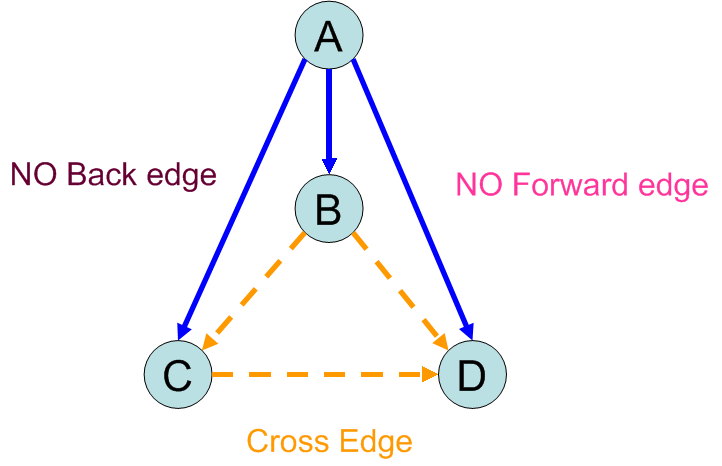
\includegraphics[scale=0.20]{figure/bfs_dfs/bfsundirected} \\ (\textcolor{red}{Cross edge})}
                & \tabincell{c}{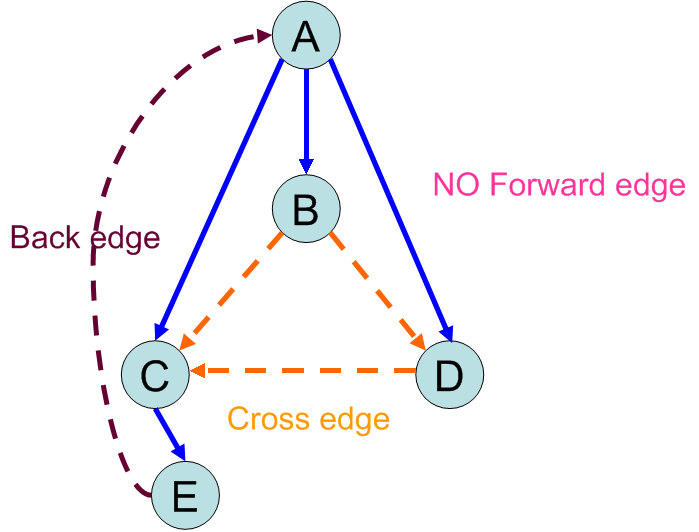
\includegraphics[scale=0.20]{figure/bfs_dfs/bfsdi} \\ (\textcolor{blue}{Back edge?})}            \\ \hline
      DFS       & \tabincell{c}{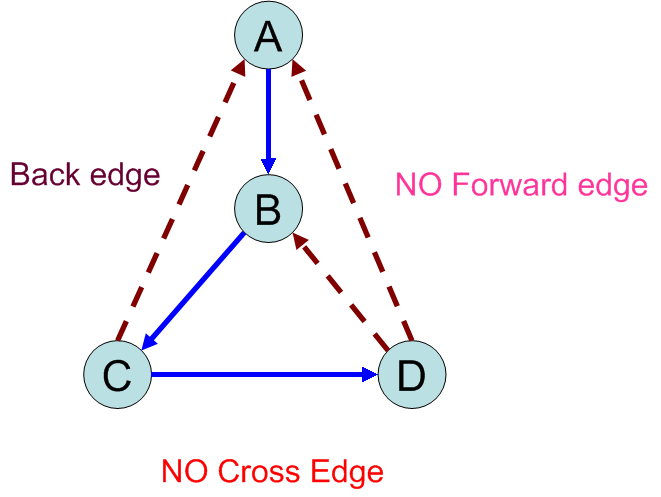
\includegraphics[scale=0.20]{figure/bfs_dfs/dfsundirected} \\ \textcolor{red}{Back edge}}
                & \tabincell{c}{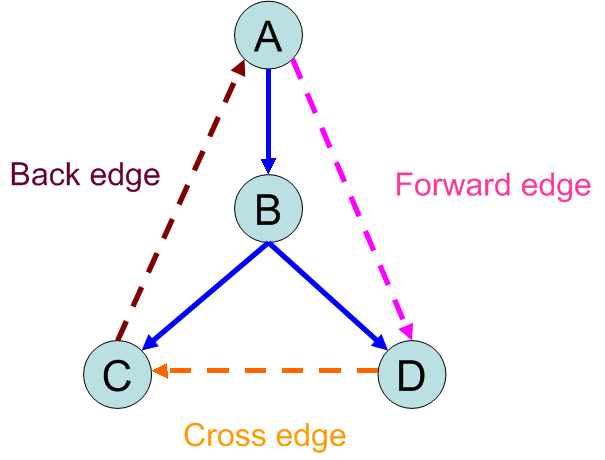
\includegraphics[scale=0.20]{figure/bfs_dfs/dfsdi} \\ \textcolor{red}{Back edge}}                              \\ \hline
    \end{tabular}
  \end{table}

\end{frame}


\begin{frame}
  \frametitle{Cycle detection problems}

  \begin{center}
    \textcolor{purple}{Using BFS on undirected graph for cycle detection:}
  \end{center}

  \begin{columns}
    \begin{column}{0.50\textwidth}
      \begin{figure}
        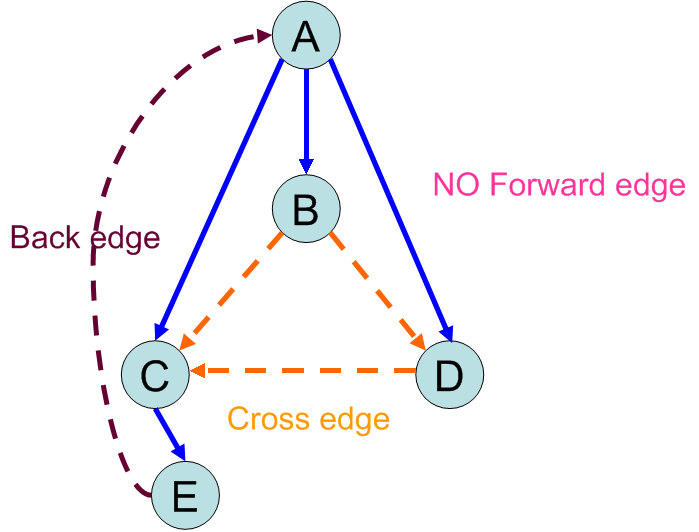
\includegraphics[scale=0.30]{figure/bfs_dfs/bfsdi}
        \caption{{\scriptsize BFS on digraph with back edges.}}
        \label{fig:bfsundirected}
      \end{figure}
    \end{column}

    \begin{column}{0.50\textwidth}
      \begin{figure}
        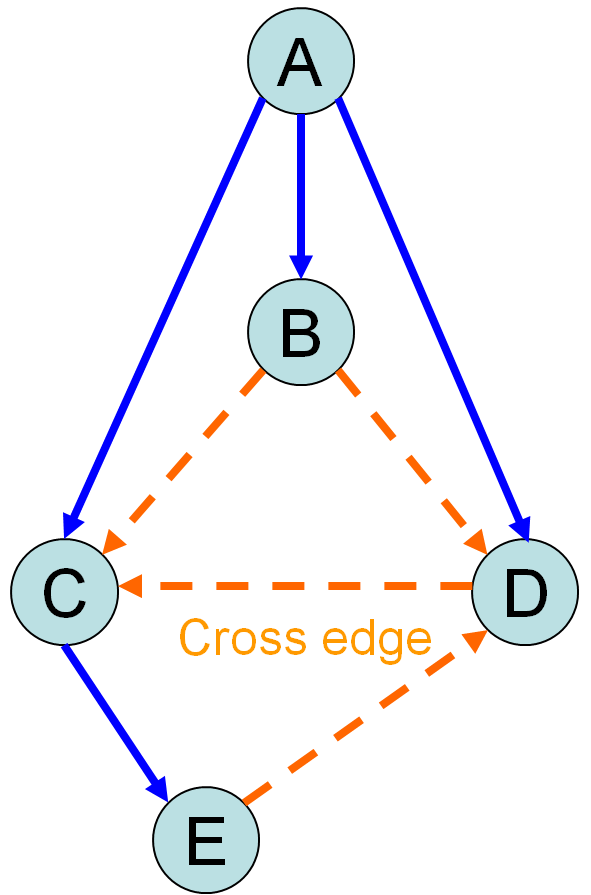
\includegraphics[scale=0.30]{figure/bfs_dfs/bfsdinoback}
        \caption{{\scriptsize BFS on digraph without back edges.}}
        \label{fig:bfsdinoback}
      \end{figure}
    \end{column}
  \end{columns}

\end{frame}




    %%%%%%%% Exploring types of edges on both BFS and DFS %%%%%%%
\subsection{Exploring DFS's Active Intervals}

\begin{frame}
  \frametitle{Exploring DFS's active intervals}

    \begin{figure}
      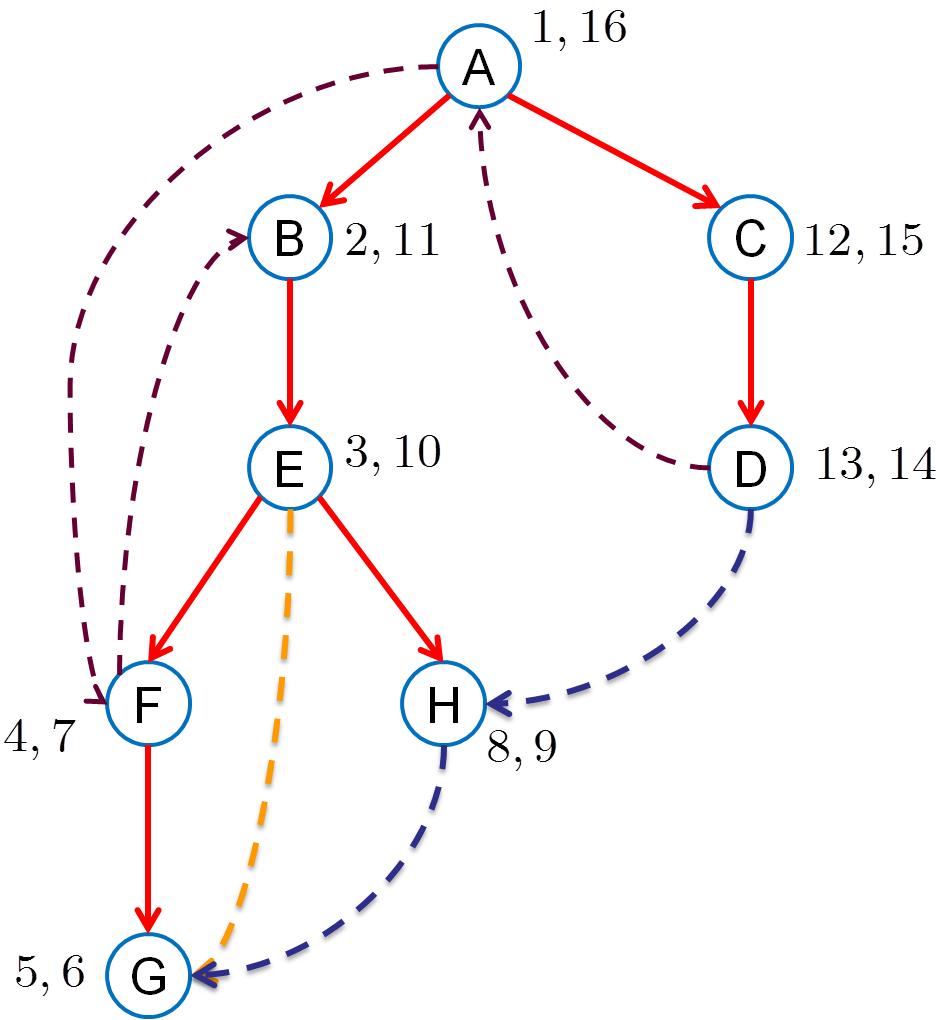
\includegraphics[scale=0.40]{figure/bfs_dfs/activeinterval}
      \caption{{\scriptsize Active intervals in DFS on digraph.}}
      \label{fig:activeinterval}
    \end{figure}

\end{frame}


\begin{frame}
  \frametitle{Exploring DFS's active intervals}

  \begin{enumerate}
    \item Who is ancestor ?
    \item How many descendants ?
      \pause
    \item topological sorting (on digraph)
    \item strongly-connected components (on digraph)
    \item biconnected components (on undirected graph)
  \end{enumerate}

\end{frame}


\subsubsection{DAG and Topological Sorting}
\begin{frame}
  \frametitle{DAG and topological sorting}

  \begin{enumerate}
    \setlength{\itemsep}{0.20cm}

    \item absence of back edges = acyclicity (DAG)
    \item topological sorting
      \begin{itemize}
        \item source, sink
      \end{itemize}
  \end{enumerate}

  \begin{figure}
    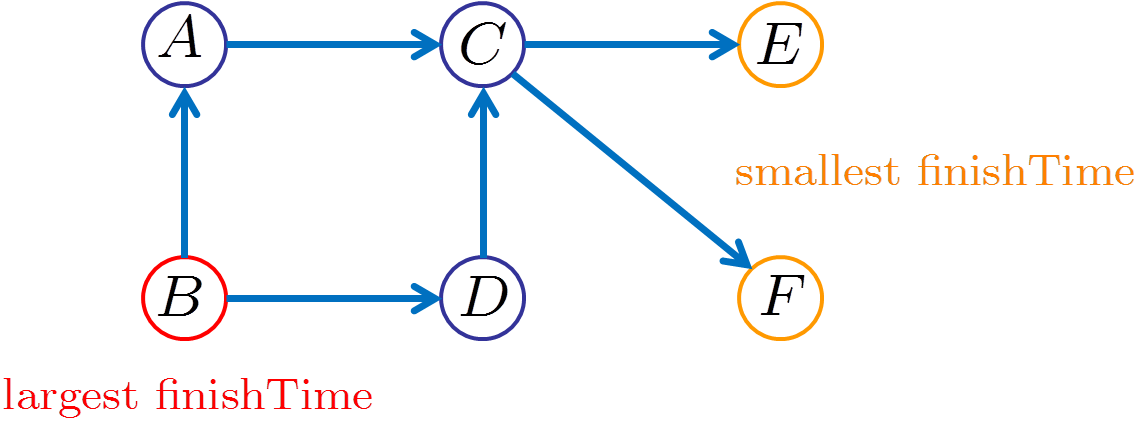
\includegraphics[scale=0.40]{figure/bfs_dfs/DAG}
    \caption{{\scriptsize Example of DAG.}}
    \label{fig:activeinterval}
  \end{figure}
      
\end{frame}

%    \item critical path
%      \begin{itemize}
%        \item longest path in DAG
%      \end{itemize}

%\begin{frame}
%  \frametitle{DAG and Topological Sorting}
%
%  \begin{columns}
%    \begin{column}{0.40\textwidth}
%      \begin{figure}
%        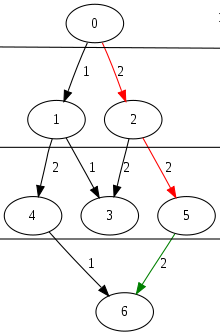
\includegraphics[scale=0.30]{figure/bfs_dfs/longestpath}
%        \caption{{\scriptsize DAG with distance layers.}}
%        \label{fig:longestpath}
%      \end{figure}
%    \end{column}
%
%    \begin{column}{0.60\textwidth}
%      \begin{figure}
%        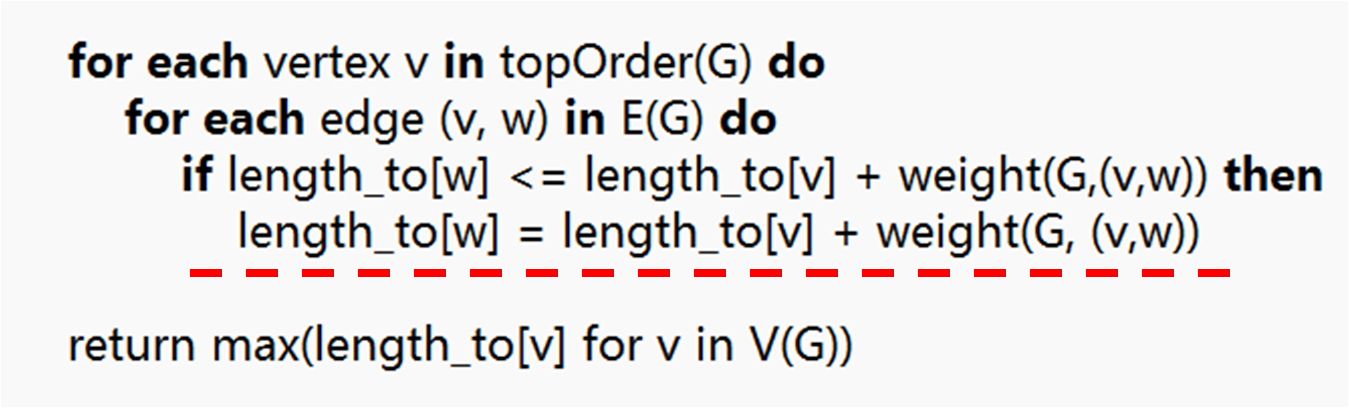
\includegraphics[scale=0.30]{figure/bfs_dfs/longestpathalg}
%        \caption{{\scriptsize Dag longest path algorithm.}}
%        \label{fig:longestpathalg}
%      \end{figure}
%    \end{column}
%
%  \end{columns}
%
%    \pause
%    \textcolor{purple}{In general graphs, longest path problem is NP-hard.}
%
%\end{frame}

\begin{frame}
  \frametitle{DAG and topological sorting}
  
  \begin{itemize}
    \item critical path $\to$ longest path in DAG
  \end{itemize}
  
  \pause
  \vspace{0.50cm}
  
  \textcolor{purple}{Note: In general graphs, longest path problem is NP-hard !}
    
\end{frame}

\subsubsection{Strongly Connected Components of a Digraph}

\begin{frame}
  \frametitle{SCC of digraph}

  \textcolor{purple}{``Two-trier'' structure of digraph} ([\textcolor{blue}{$P_{379}$ 7.22}]):

  \begin{figure}
    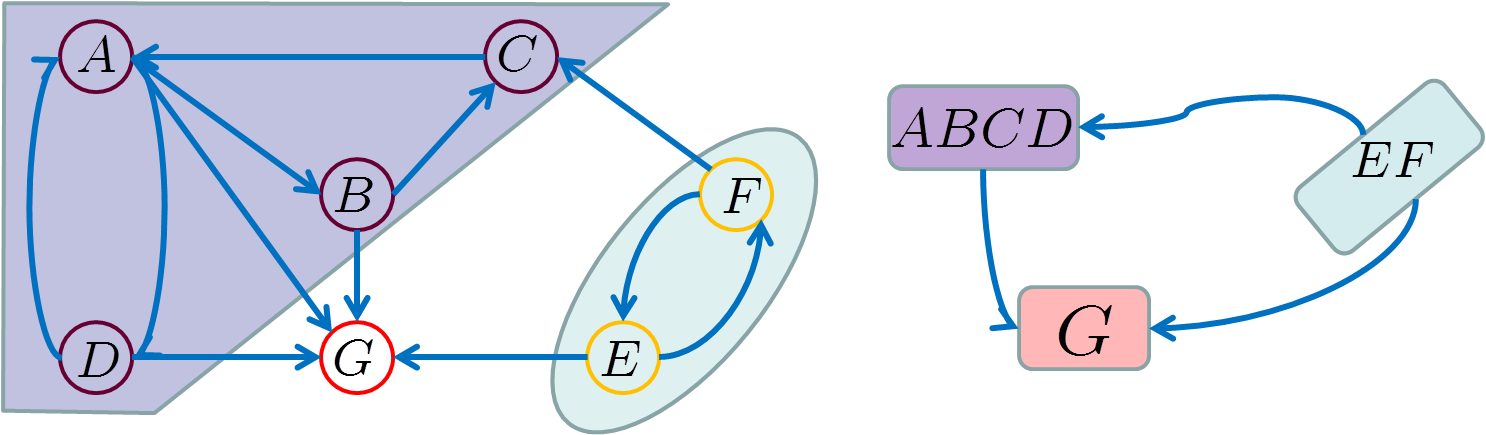
\includegraphics[scale=0.35]{figure/bfs_dfs/SCCDI}
    \label{fig:scc}
  \end{figure}

  \pause

{\small

  \begin{enumerate}
    \item ``The node that has \textcolor{red}{highest} finishTime in DFS must lie in a \textcolor{red}{source SCC''};
    \pause
    \item What we need is sink! So try \textcolor{red}{$G^R$}; ([\textcolor{blue}{$P_{380}$ 7.26}])
    \item When a sink SCC is found (by connectivity), just delete it and continue \textcolor{red}{recursively}.
  \end{enumerate}
}

\end{frame}


\subsubsection{Biconnected Components of an Undirected Graph}

\begin{frame}
  \frametitle{Biconnected components of an undirected graph}

  \textcolor{purple}{Algorithms for biconnected components:}
  \begin{description}
    \setlength{\itemsep}{0.20cm}
    \item [Brute force:] try every vertex and check connectivity: $O \big( n(m+n) \big )$.
    \item [Clever approach:] single DFS making use of \textcolor{blue}{\emph{back edges and active intervals}}.
  \end{description}

\end{frame}


\begin{frame}
  \frametitle{Biconnected components of an undirected graph}

    \begin{columns}
      \begin{column}{0.50\textwidth}
         \begin{figure}
            \begin{center}
              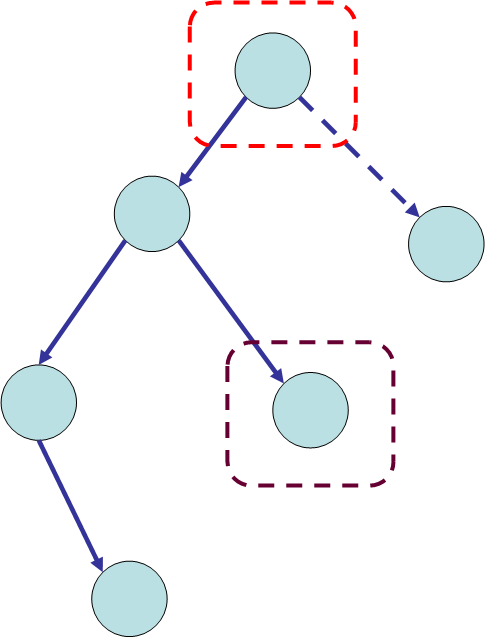
\includegraphics[scale=0.30]{figure/bfs_dfs/dfsbiconn}
              \caption{What if DFS tree is the entirety of the graph ?}
              \label{fig:dfsbiconn}
            \end{center}
          \end{figure}
      \end{column}

      \begin{column}{0.50\textwidth}
          \begin{figure}
            \begin{center}
              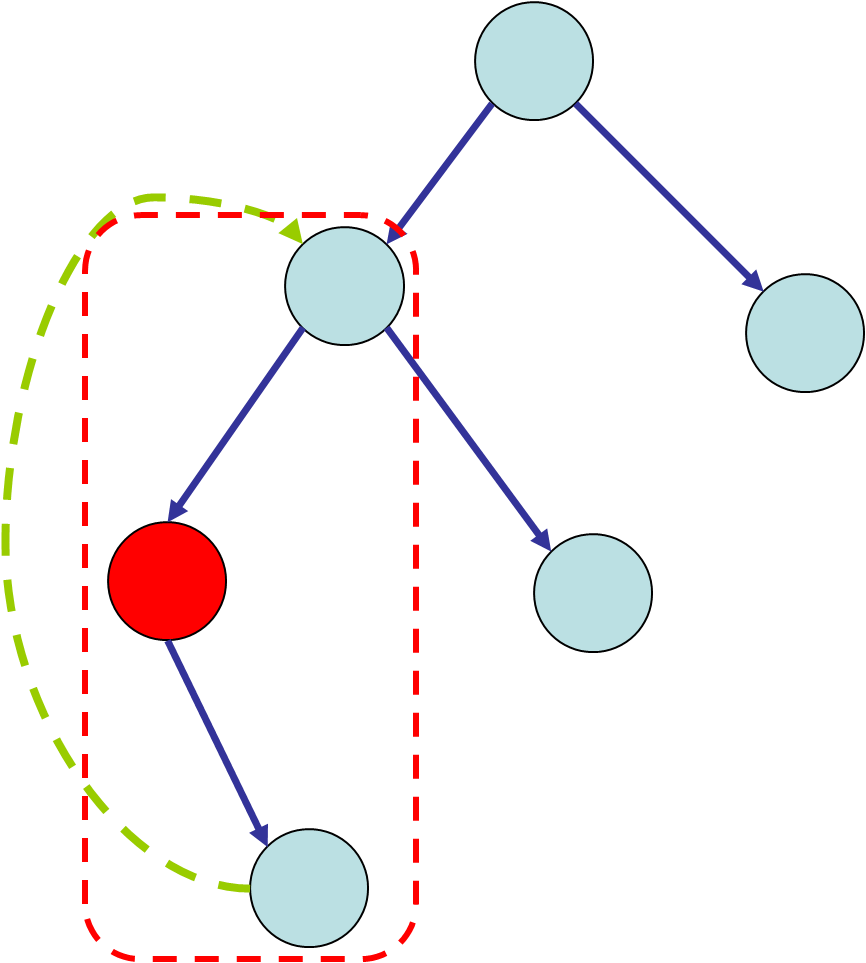
\includegraphics[scale=0.30]{figure/bfs_dfs/backedgebiconn}
              \caption{Back edge, cycle, no articulation vertices.}
              \label{fig:backedgebiconn}
            \end{center}
          \end{figure}
      \end{column}

    \end{columns}

\end{frame}


%\begin{frame}
%  \frametitle{Biconnected components of an undirected graph}
%
%  \textcolor{purple}{Important information:}
%
%  \textcolor{blue}{the extend to which back edges link chunks of the DFS tree back to ancestor nodes:}
%  \begin{enumerate}
%    \setlength{\itemsep}{0.20cm}
%
%    \item $v$ is first discovered.
%        \[
%          back = discoverTime(v).
%        \]
%    \item back edge $vw$.
%        \[
%          back = min(back, discoverTime(w)).
%        \]
%    \item backtracking from $w$ to $v$.
%        \[
%          back = min(back, wback).
%        \]
%  \end{enumerate}
%
%\end{frame}


\begin{frame}
  \frametitle{Biconnected components of an undirected graph}
  
  \begin{figure}
    \begin{center}
      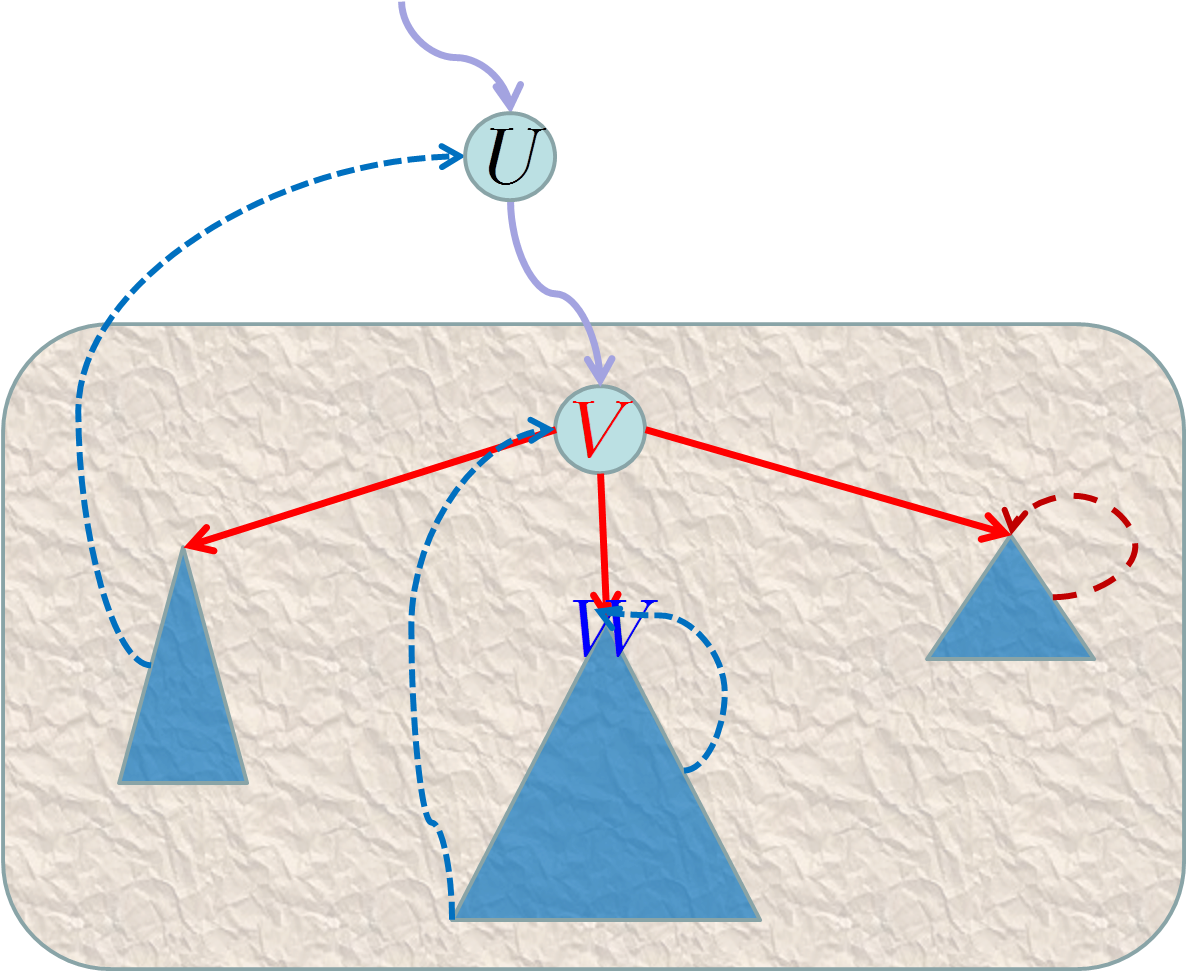
\includegraphics[scale=0.40]{figure/bfs_dfs/bicon1}
      \caption{{\scriptsize Three cases of articulations (1).}}
      \label{fig:bicon1}
    \end{center}
  \end{figure}  
  
\end{frame}


\begin{frame}
  \frametitle{Biconnected components of an undirected graph}

  \begin{figure}
    \begin{center}
      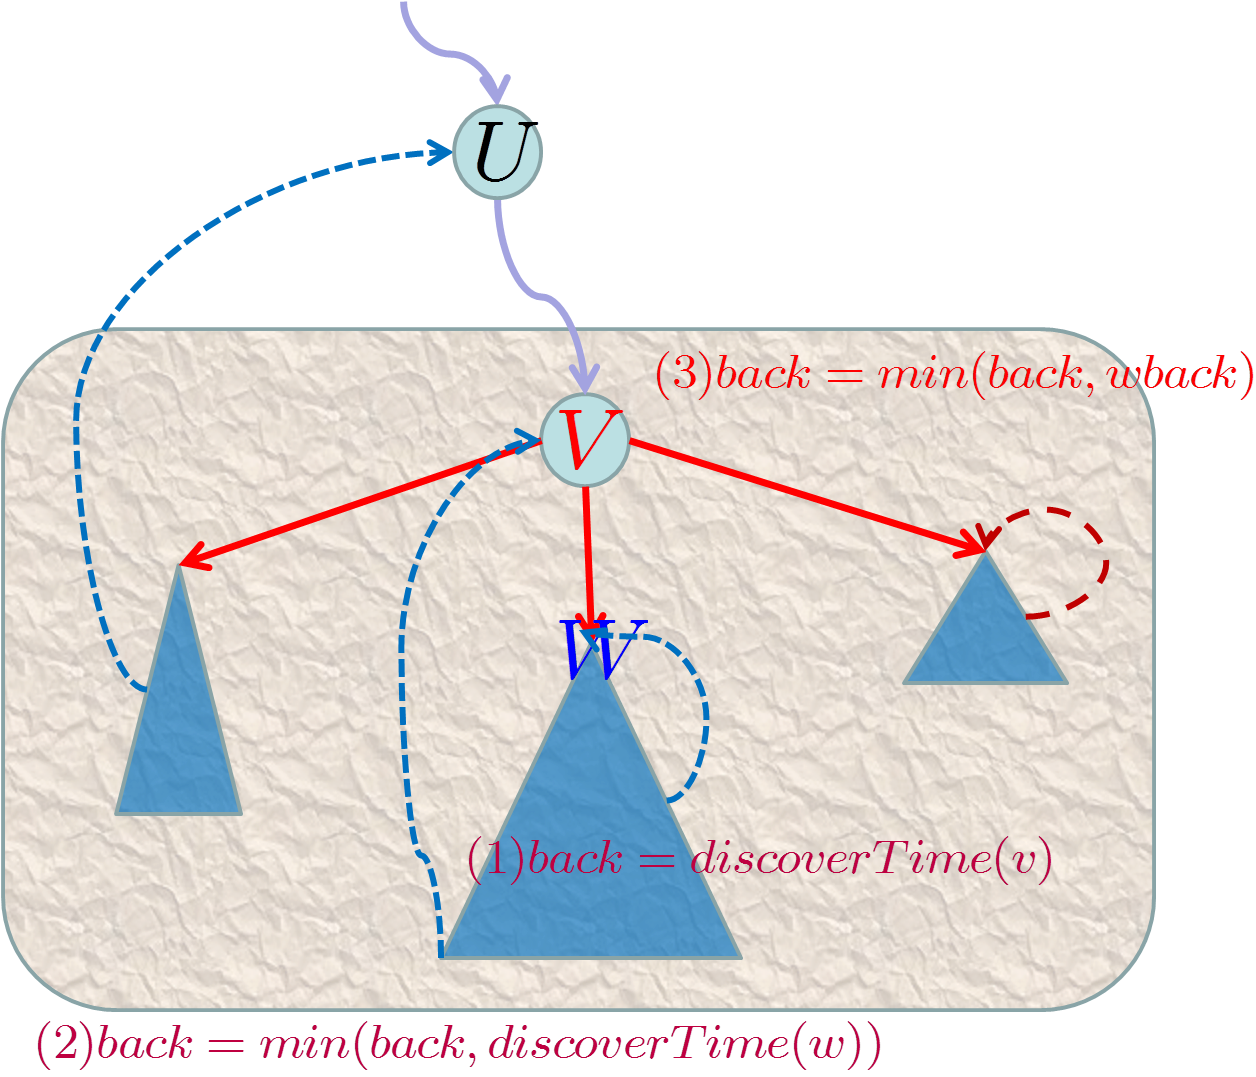
\includegraphics[scale=0.40]{figure/bfs_dfs/bicon2}
      \caption{{\scriptsize Three cases of articulations (2).}}
      \label{fig:bicon2}
    \end{center}
  \end{figure}

\end{frame}


\begin{frame}
  \frametitle{Biconnected components of an undirected graph}

  \begin{figure}
    \begin{center}
      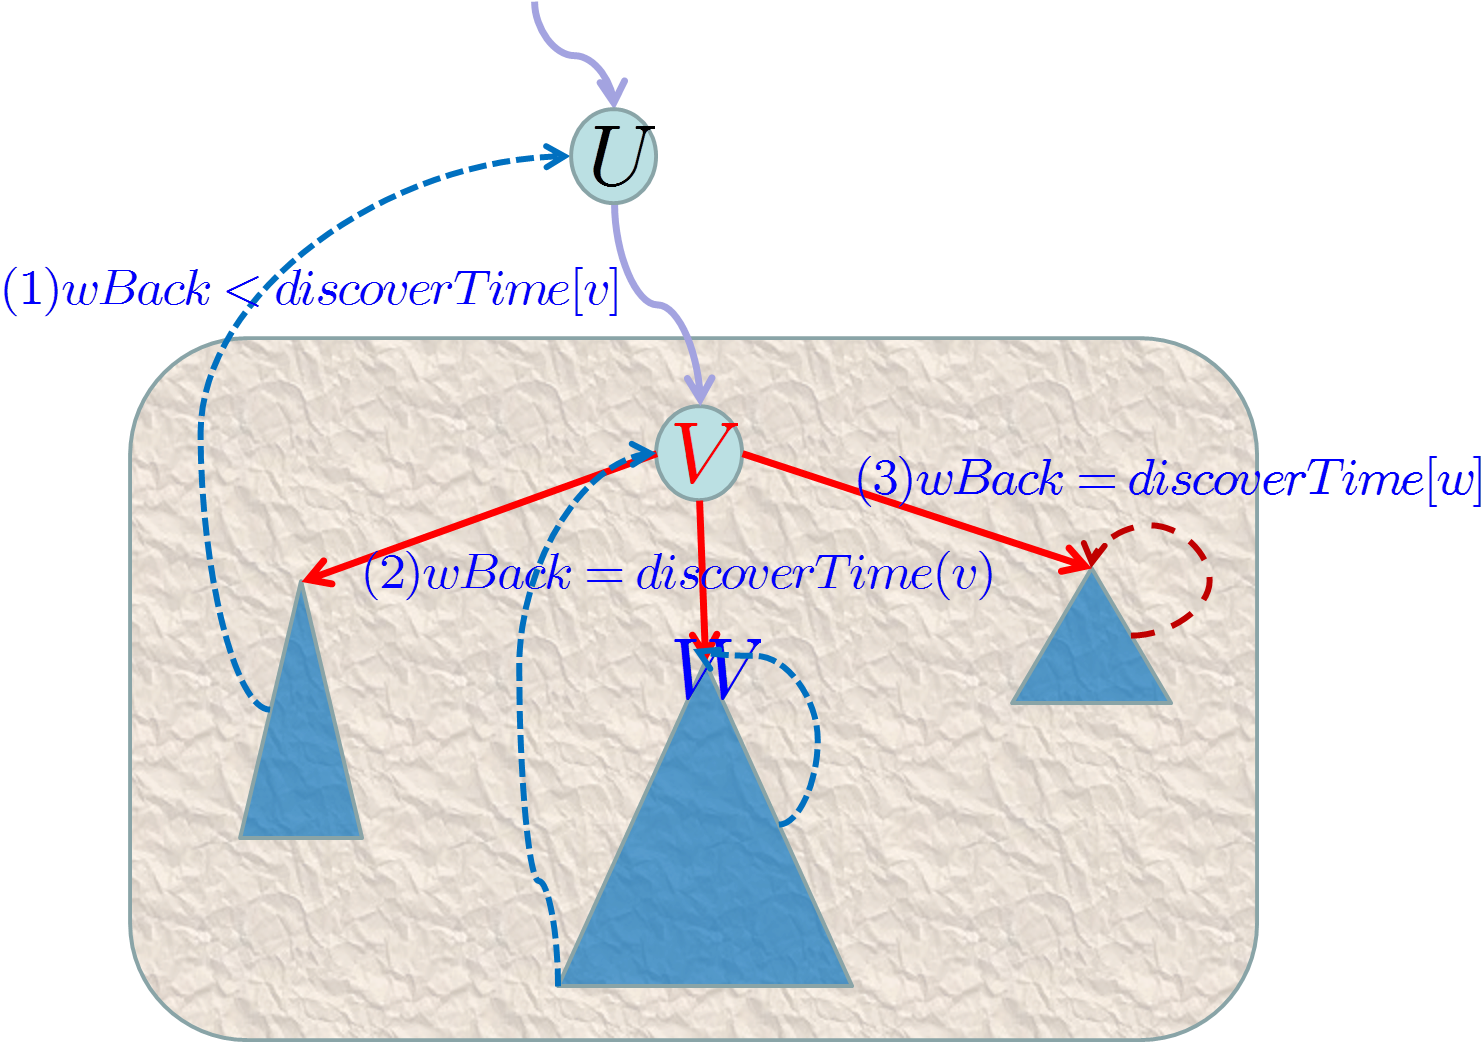
\includegraphics[scale=0.40]{figure/bfs_dfs/bicon3}
      \caption{{\scriptsize Three cases of articulations (3).}}
      \label{fig:bicon3}
    \end{center}
  \end{figure}

\end{frame}



\begin{frame}
  \frametitle{Biconnected components of an undirected graph}

  \begin{figure}
    \begin{center}
      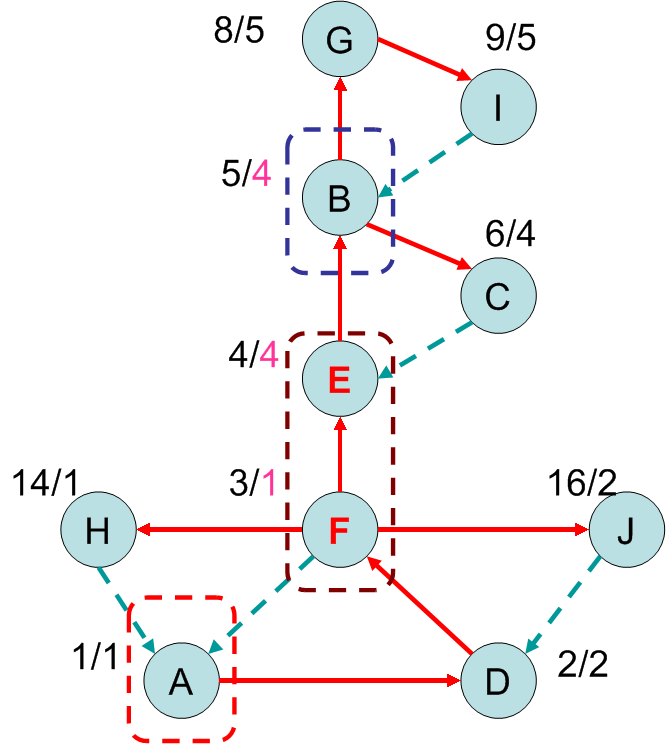
\includegraphics[scale=0.30]{figure/bfs_dfs/articulationex}
      \caption{Three cases of articulations.}
      \label{fig:articulations}
    \end{center}
  \end{figure}

\end{frame}


\begin{frame}
  \frametitle{Biconnected components of an undirected graph}

  \textcolor{purple}{Q:} How the reachability relation impacts whether $v$ is an articulation vertex ?
  \begin{enumerate}
    \item Root cut-nodes ([\textcolor{blue}{$P_{382}$ 7.37}]).
    \item Bridge cut-nodes.
    \item Parent cut-nodes.
  \end{enumerate}

  \pause
  \vspace{0.40cm}

    Q : $\textrm{Back } \ge \textrm{discoverTime} \lbrack v \rbrack$ ([\textcolor{blue}{$P_{383}$ 7.42}]).

  \pause

    A : $\textrm{Back } = \textrm{discoverTime} \lbrack v \rbrack$. It just detects Bridge cut-nodes.

\end{frame} 